\chapter{Mount}
\label{chapter:mount}

\section{Description}

The mount is an ASTELCO NTM-500 German equatorial mount. For details, see the ASTELCO manual. 

\subsection{Mount}

The mount itself is obviously located at the top of the telescope pier.
Figure~\ref{figure:mount-panel} shows the mount panel.

\begin{figure*}
\begin{center}
\resizebox{\columnwidth}{!}{%
\begin{labeled}{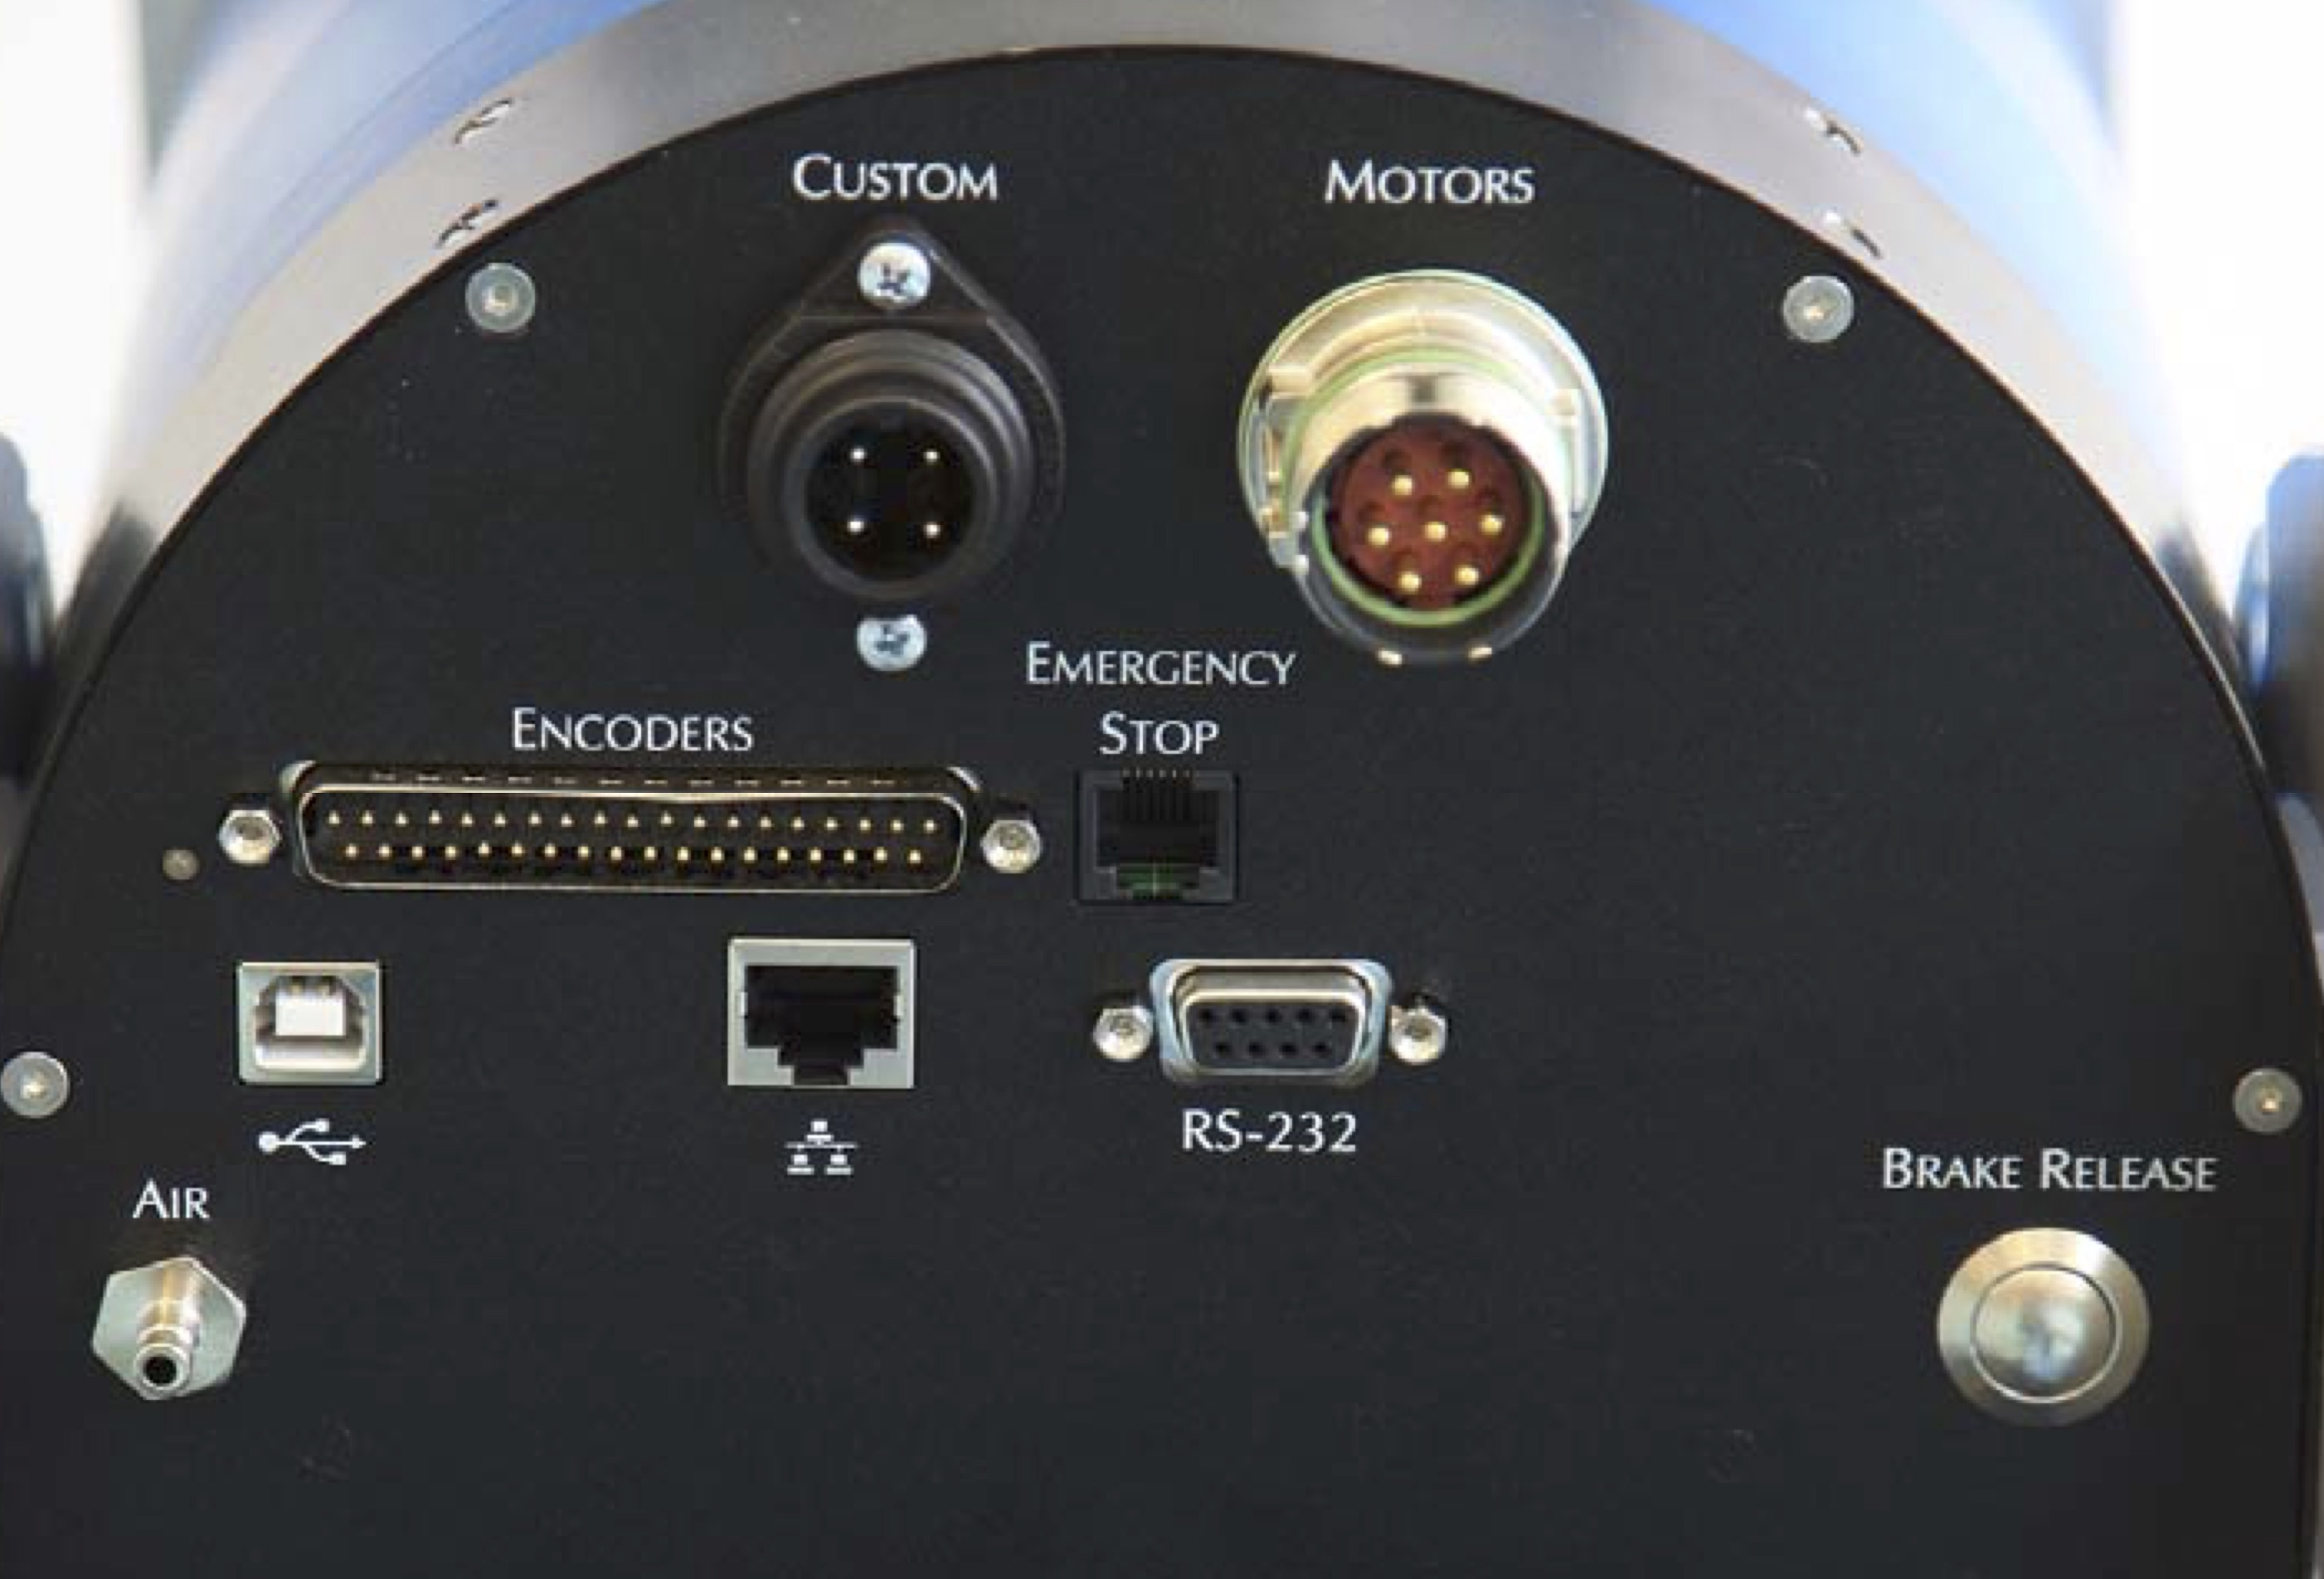
\includegraphics[width=\linewidth]{figures/mount-panel.jpg}}
\arrowandlabel{(+7.3,-2.0)}{(+7.3,-3.0)}{west}{Break Release};
\end{labeled}}
\end{center}
\caption{The mount panel showing the break release button.}
\label{figure:mount-panel}
\end{figure*}

\ifcoatli
At {\projectname} we not not pass any electrical connections through the mount. All electrical connections to the instrument and telescope pass through the flexible cable chain.
\fi

\ifddoti
At {\projectname} we pass 127~VAC and network connections through the mount HA axis up to Box D. The 127~VAC supply uses the “CUSTOM” connector. We also pass 127~VAC and network connections through the mount declination axis from Box D to Box E.
\fi

\subsection{Mount Controller}

The mount controller is a cream 4U box located in the rack in the shed. 
Figure~\ref{figure:mount-controller-panel} shows the controller front panel, with the connectors and the power, fan alarm reset, and factory reset buttons.

The mount controller is connected to the mount by two cables (one for the motors and another for the encoders) and a compressed air hose (for the brakes). It is also connected to a GPS receiver which is located on the
\ifcoatli
south-west side
\fi
\ifddoti
south-east side
\fi
of the shed.

The mount controller is connected to circuit B, through the 127~V UPS and iBootBar. (The mount controller should not be connected to 220~VAC.)

\begin{figure*}
\begin{center}
\resizebox{\columnwidth}{!}{%
\begin{labeled}{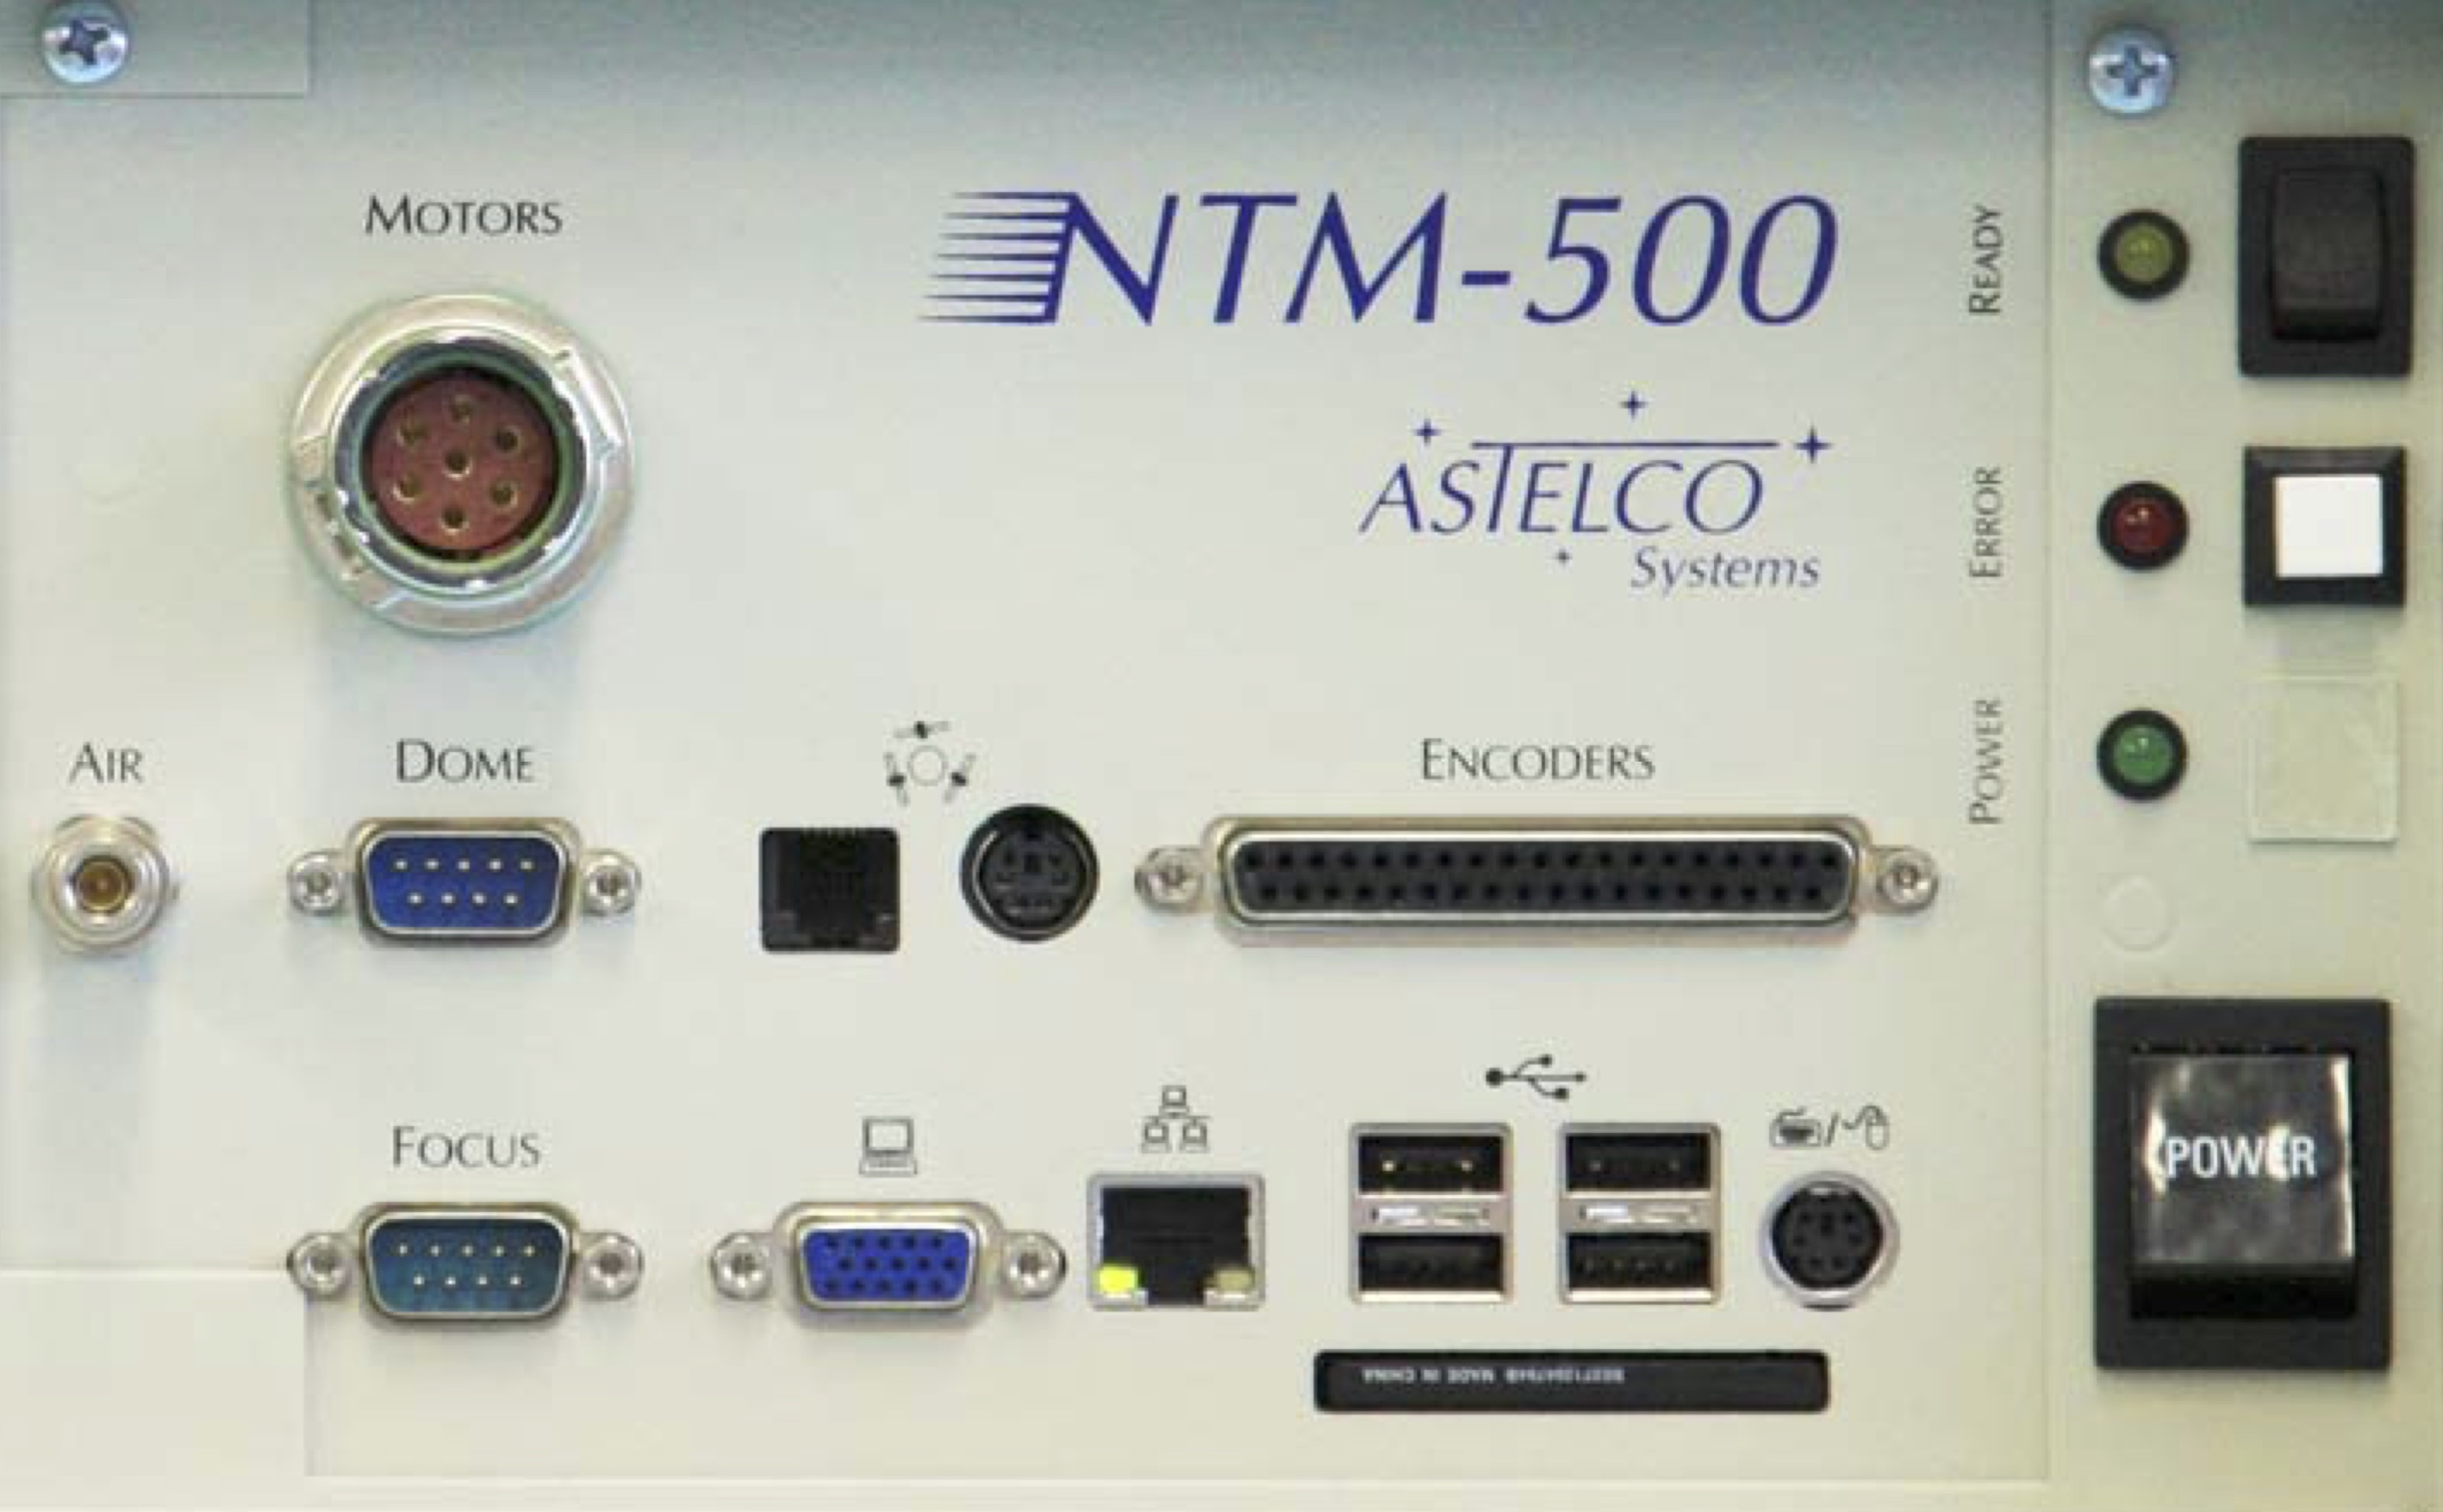
\includegraphics[width=\linewidth]{figures/mount-controller-panel.jpg}}
\arrowandlabel{(+6.2,+2.5)}{(+7.5,+2.5)}{west}{Factory Reset};
\arrowandlabel{(+6.2,+1.1)}{(+7.5,+1.1)}{west}{Fan Alarm Reset};
\arrowandlabel{(+6.2,-2.0)}{(+7.5,-2.0)}{west}{Power};
\end{labeled}}
\end{center}
\caption{The mount controller front panel showing the connectors and the power, fan alarm reset, and factory reset buttons.}
\label{figure:mount-controller-panel}
\end{figure*}

\section{Maintenance Procedures}

\subsection{Manually Moving the Mount}

Press the BRAKE button on the panel on the south side of the mount. While this button is pressed, the brakes on both axes will be released and you can move the telescope by hand. 

Sometimes, especially after an error, the mount takes a while to recover and you need to press and hold the button for up to a minute before the brakes are released.

\subsection{Manually Switching Off}
\label{section:mount-power-off}

Press the power button on the front panel (shown in Figure~\ref{figure:mount-controller-panel}). Do not confuse the power button with the factory reset button! The power button is in the lower right and the factory reset in the upper right.

\subsection{Manually Switching On}
\label{section:mount-power-on}

Press the power button on the front panel (shown in Figure~\ref{figure:mount-controller-panel}). Do not confuse the power button with the factory reset button! The power button is in the lower right and the factory reset in the upper right.


\section{Bibliography}

\begin{flushleft}
\begin{itemize}
\item “\href{technical-manual/bibliography/astelco-mount-ntm-manual.pdf}{NTM Technical Reference Manual}”, ASTELCO, Version 3.7.
\item “\href{technical-manual/bibliography/astelco-mount-ntm-technical-description.pdf}{NTM Technical Description}”, ASTELCO, Version 3.7.
\item “\href{bibliography/astelco-opentci.pdf}{OpenTCI}”, ASTELCO, Version 2.5.
\item “\href{bibliography/astelco-tpl2.pdf}{TPL2}”, ASTELCO, Version 2.0.
\item “\href{bibliography/astelco-mount-drawing-5824.pdf}{Drawing 5824 -- Mount column interface}”, ASTELCO.
\item “\href{bibliography/astelco-mount-drawing-ntm-base-plate.pdf}{Drawing -- NTM Base Plate}”, ASTELCO.
\item “\href{bibliography/astelco-mount-drawing-ntm-dimensions.pdf}{Drawing -- NTM Dimensions}”, ASTELCO.
\item “\href{bibliography/tau-tec-ascom.pdf}{TCLM/TPL2 ASCOM Driver User Manual}”, Tau-tec, 2010
\end{itemize}
\end{flushleft}
